\documentclass[11pt,a4paper]{article}
\usepackage[utf8]{inputenc}
\usepackage[T1]{fontenc}
\usepackage{lmodern}
\usepackage{microtype}
\usepackage[margin=2.4cm]{geometry}
\usepackage{amsmath,amssymb,bm}
\usepackage{graphicx}
\usepackage{float}
\usepackage{booktabs,tabularx,longtable}
\usepackage[table]{xcolor}
\usepackage{enumitem}
\usepackage[most]{tcolorbox}
\usepackage{caption}
\usepackage{titlesec}
\usepackage{fancyhdr}
\usepackage[hidelinks]{hyperref}
\usepackage{cleveref}

\definecolor{accent}{HTML}{23606B}
\definecolor{soft}{HTML}{E6F0F1}
\definecolor{warn}{HTML}{9A5A12}
\definecolor{warnsoft}{HTML}{FBF0E2}

\setlist[itemize]{nosep, leftmargin=*, topsep=3pt}
\setlist[enumerate]{nosep, leftmargin=*, topsep=3pt}
\captionsetup{font=small, labelfont=bf}
\titleformat{\section}{\Large\bfseries\color{accent}}{\thesection}{0.8em}{}
\titleformat{\subsection}{\large\bfseries}{\thesubsection}{0.7em}{}
\setlength{\parskip}{4pt}
\renewcommand{\arraystretch}{1.18}

\pagestyle{fancy}
\fancyhf{}
\fancyhead[L]{\small Paper 1 on a realistic quadrotor model}
\fancyhead[R]{\small Phase 2 report}
\fancyfoot[C]{\thepage}

\newtcolorbox{keybox}[1][]{colback=soft, colframe=accent, boxrule=0.6pt, arc=2pt, left=6pt, right=6pt, top=4pt, bottom=4pt, fonttitle=\bfseries, #1}
\newtcolorbox{cavbox}[1][]{colback=warnsoft, colframe=warn, boxrule=0.6pt, arc=2pt, left=6pt, right=6pt, top=4pt, bottom=4pt, fonttitle=\bfseries, #1}

\newcommand{\R}{\mathbb{R}}
\newcommand{\ethree}{\mathbf{e}_3}
\newcommand{\code}[1]{\texttt{\small #1}}

\begin{document}

\begin{titlepage}
\centering
\vspace*{2.5cm}
{\color{accent}\rule{\textwidth}{1.2pt}}\\[14pt]
{\LARGE\bfseries Geometric Control of a Cable-Suspended Payload\\[4pt] on a Realistic Quadrotor Model}\\[10pt]
{\large Reproduction and stress test of Sreenath, Lee \& Kumar (CDC 2013)\\ in MuJoCo with the Skydio X2}\\[14pt]
{\color{accent}\rule{\textwidth}{1.2pt}}\\[1.6cm]
{\large Haidar Saad}\\[4pt]
Master's research, advisor Prof.\ Andry\\[1.2cm]
{\large Phase 2 report}\\[4pt]
November 2026\\[2.2cm]
\begin{minipage}{0.82\textwidth}\small
\textbf{How to read this document.} It is written for someone who wants to study the work, not only see the
results: every modelling choice is explained with its reason, every result is traced to the experiment that produced
it, and \Cref{app:reproduce} lists the commands that regenerate each number. Code and result folders are in the
public repository \url{https://github.com/haidar996/suspended-payload-trajectory-tracking}.
\end{minipage}
\end{titlepage}

\tableofcontents
\newpage

% =====================================================================================================
\section*{Summary}
\addcontentsline{toc}{section}{Summary}

A quadrotor carrying a load on a cable is an underactuated system: the four rotors act on the drone, and the load
moves only through the cable. Sreenath, Lee and Kumar (CDC 2013), called \emph{Paper~1} here, showed that this system
is differentially flat with the load position and the drone yaw as flat outputs, and designed a geometric controller
that tracks the load position with almost-global stability guarantees. Their proofs and simulations assume a rigid
massless cable that is always taut, unlimited rotor thrust, perfect state knowledge and instantaneous actuators.

We reimplemented the flatness map and the controller from the equations of the paper and ran them on a realistic
simulated drone, the Skydio X2 from MuJoCo Menagerie, whose four rotors each produce between 0 and 13~N. Under the
paper's own assumptions every result reproduces: the flatness map agrees with an independent implementation to
$10^{-13}$, references are tracked to below 0.2~mm, and the drone recovers from a $178^\circ$ flip. We then removed
the assumptions one at a time, and each removal broke something specific:

\begin{itemize}
\item Rotor limits cap the attitude loop at about 30~rad/s, give the X2 a maximum speed on the paper's own ellipse
  (period $T_0^\ast = 2.12$~s), and make recovery from flips of $20^\circ$ or more chaotic.
\item A cable that can go slack makes the $178^\circ$ recovery diverge, even with unlimited thrust: the paper's
  recovery depends on the cable pushing the load.
\item With the published gain scaling, a 1~m cable crashes the X2 on a $15^\circ$ initial swing.
\item Motion-capture-level velocity noise crashes every run, because the controller differentiates noisy
  states without an estimator; a 35~ms motor lag breaks swing recovery, and gains slow enough for the lag can no longer
  damp the swing.
\end{itemize}

These results define the gaps that the next phases address: control that respects rotor limits, recovery that
handles a slack cable, state estimation, and swing damping that is compatible with motor lag.

% =====================================================================================================
\section{Introduction}

\subsection{Problem}
Transporting a suspended load with a multirotor is attractive because the cable keeps the load away from the rotors and
lets a small drone carry objects of many shapes. The price is a coupled, underactuated dynamics: the drone has six
degrees of freedom and four inputs, and the load adds two more degrees of freedom (the direction of the cable) with no
input of their own. Moving the drone makes the load swing; letting the load swing makes the drone's position hard to
hold. The research question of this project is how to make the \emph{load} follow a desired trajectory accurately and
robustly, eventually with learning-based methods, under realistic conditions.

\subsection{Why reproduce Paper 1 first}
Paper~1 is the reference model-based solution. Its two ideas, differential flatness and geometric control on
$SO(3)\times S^2$, are used by most later work, including the reinforcement-learning papers planned for the later
phases. Reproducing it gives us (i) a verified simulation framework, (ii) a strong baseline, and (iii) a map of where
the classical theory stops working, which is where a contribution can be made.

\subsection{Working method}
The project follows a fixed research workflow: before any implementation, the literature is searched for each modelling
choice; the choice is discussed and agreed; it is recorded in a design log (\code{SIMULATION\_DESIGN.md}, decisions
D1--D12 and findings F1--F10); and implementation then proceeds in small steps, each with explicit pass/fail gates,
automated tests, and a commit only after approval. Every experiment writes a self-contained result folder with its
configuration, git commit, metrics, raw data and figures. This report summarises Phase~1 (simulation core) and
Phase~2 (Paper~1).

% =====================================================================================================
\section{Background: model, flatness and controller of Paper 1}
\label{sec:theory}

\subsection{System model}
We use the notation of Paper~1. The drone has mass $m_Q$, inertia $J$ about its centre of mass, position $x_Q\in\R^3$,
attitude $R\in SO(3)$ and body angular velocity $\Omega$. The load is a point mass $m_L$ at $x_L$, attached by a
massless cable of length $l$ at the drone's centre of mass. The unit vector $q\in S^2$ points from the drone to the load,
so $x_Q = x_L - l\,q$, and $\omega = q\times\dot q$ is the cable's angular velocity. The rotors produce a collective
thrust $f$ along the body axis $R\ethree$ and a body moment $M$. While the cable is taut with tension $T$,
\begin{align}
m_L(\ddot x_L + g\ethree) &= -T q, \label{eq:load}\\
m_Q(\ddot x_Q + g\ethree) &= f R\ethree + T q, \label{eq:quad}\\
J\dot\Omega + \Omega\times J\Omega &= M,\qquad \dot R = R\,\hat\Omega, \label{eq:att}
\end{align}
where $\hat{\cdot}$ maps a vector to its skew-symmetric matrix. The configuration space is $SE(3)\times S^2$ and the
system has eight degrees of freedom with four inputs.

\subsection{Differential flatness}
A system is \emph{differentially flat} if a set of outputs (the flat outputs) exists such that all states and inputs are
algebraic functions of these outputs and finitely many of their derivatives. For this system the flat outputs are the load
position $x_L$ and the drone yaw $\psi$. The map, implemented in \code{sim/flatness.py}, is:
\begin{align}
u &= \ddot x_L + g\ethree,\qquad q = -u/\|u\|,\qquad T = m_L\|u\|, \\
F &= f R\ethree = (m_Q+m_L)\,u - m_Q l\,\ddot q,\\
b_3 &= F/\|F\|,\quad R = [\,b_1\; b_2\; b_3\,] \text{ from } b_3 \text{ and } \psi,\\
\Omega &= (R^\top\dot R)^\vee,\qquad M = J\dot\Omega + \Omega\times J\Omega .
\end{align}
The attitude needs the fourth derivative of $x_L$ (through $\ddot q$), the body rate the fifth and the moment the sixth.
The map is singular when $\|u\|\to 0$ (the load in free fall, zero tension) and when the thrust direction is parallel
to the yaw heading.

\textbf{Exact derivatives by jet arithmetic.} Instead of symbolic algebra (too slow, 7~ms per evaluation) or
finite differences (inaccurate at sixth order), we propagate truncated Taylor series (``jets'') through the map. A jet
stores a value and its first $n$ derivatives; products use the Leibniz rule and normalisation uses the series of
$1/\sqrt{\cdot}$. All six derivatives are then exact to round-off at 0.1~ms per evaluation (\code{sim/jet.py}).

\subsection{Geometric controller}
Paper~1 builds three flight modes, each on top of the previous one. Our implementation is
\code{sim/controllers/geometric\_paper1.py}.

\textbf{(a) Drone attitude (Eq.~21 of Paper~1).} With attitude error $e_R=\tfrac12(R_d^\top R - R^\top R_d)^\vee$ and
rate error $e_\Omega = \Omega - R^\top R_d\Omega_d$,
\begin{equation}
M = -K_R e_R - K_\Omega e_\Omega + \Omega\times J\Omega - J\big(\hat\Omega R^\top R_d\Omega_d - R^\top R_d\dot\Omega_d\big).
\end{equation}

\textbf{(b) Cable attitude (Eqs.~25--32).} With cable errors $e_q = \hat q^2 q_d$ and
$e_{\dot q} = \dot q - (q_d\times\dot q_d)\times q$ (a tangent vector at $q$), the desired thrust vector is
\begin{equation}
F = F_n - F_{pd} - F_{ff},\qquad F_{pd} = -k_q e_q - k_\omega e_{\dot q},
\end{equation}
with feed-forward $F_{ff}= m_Q l\,\langle q, q_d\times\dot q_d\rangle\,(q\times\dot q) + m_Q l\,(q_d\times\ddot q_d)\times q$.
The commanded attitude $R_c$ has third axis $F/\|F\|$, and $f = F\cdot R\ethree$.

\textbf{(c) Load position (Eqs.~36--38).} With $e_x = x_L - x_{L,d}$ and $e_v = \dot x_L - \dot x_{L,d}$,
\begin{equation}
A = -k_x e_x - k_v e_v + (m_Q+m_L)(\ddot x_{L,d} + g\ethree) + m_Q l\,\langle\dot q,\dot q\rangle q,\qquad
q_c = -A/\|A\|,\qquad F_n = \langle A, q\rangle q .
\end{equation}

\textbf{Time-scale separation.} The stability argument treats the three loops as nested: the attitude loop is fast enough
to be at its target, the cable loop is fast relative to the position loop. In Paper~1 this is a singular-perturbation
argument with a small parameter $\varepsilon$ scaling the attitude gains. In practice it means the loop bandwidths must
be well separated, and \Cref{sec:gains} shows how much separation is needed.

\textbf{Rates of the computed commands.} Modes (b) and (c) need $\dot q_c, \ddot q_c$ and $\Omega_c, \dot\Omega_c$. We
take them from the flatness map of the reference (exact feed-forward). Two ablations, filtered numerical
differentiation and zero rates, are kept to show why this matters (\Cref{sec:k-gates}).

% =====================================================================================================
\section{Simulation framework}
\label{sec:framework}

\subsection{Design decisions}
Twelve design decisions were made from the literature before any code was written. \Cref{tab:decisions} gives the ones
used in this report; the design log contains the sources and the alternatives that were rejected.

\begin{table}[htbp]
\centering\small
\begin{tabularx}{\textwidth}{@{}l X X@{}}
\toprule
ID & Decision & Main reason \\
\midrule
D1 & Simulator: MuJoCo 3.17 (CPU now, MJX later for RL) & accurate contact-free rigid-body dynamics; same model on GPU later \\
D2 & Drone: Skydio X2 from MuJoCo Menagerie (vendored, unmodified) & no real drone available; maintained, realistic inertia and rotor layout \\
D3 & Cable models C1--C6 as an experimental variable & literature uses rigid, elastic, chained and rod models; C1 is Paper~1, C3 is Paper~3 \\
D5 & Physics 1~ms RK4; inner loop 500~Hz; outer loop 100~Hz & no contacts, so RK4 is the most accurate choice \\
D6 & Payload P1 point mass 0.2~kg (P3 rigid cylinder later) & matches Paper~1; P3 needed for Paper~3 \\
D7 & Cable length 0.5~m nominal; 0.25 and 1.0~m in sweeps & covers the range used in the literature \\
D8 & Actuation stack SRT / CTBM / CTBR; motor lag 35~ms in the main benchmark & CTBR is the interface used by RL papers and real autopilots \\
D9 & Benchmark trajectories T0--T5, metrics, success rule & no shared benchmark exists for payload control \\
D10 & Realism levels L0 (ideal), L1 (noise, delay, drag), L2 (no payload sensor) & tests reality gap step by step \\
D11 & Randomisation ranges & for robustness tests and RL training \\
D12 & Tuning protocol & fair comparison between controllers (Phase~3) \\
\bottomrule
\end{tabularx}
\caption{Design decisions referenced in this report.}
\label{tab:decisions}
\end{table}

\subsection{The Skydio X2 model}
The X2 is loaded from the Menagerie files and modified only in code (through MuJoCo's \code{MjSpec} editing API), so
the vendored files stay identical to upstream. Its properties are read back from the compiled model, never hard-coded.

\begin{table}[htbp]
\centering\small
\begin{tabular}{@{}ll@{}}
\toprule
Property & Value \\
\midrule
Mass $m_Q$ & 1.325 kg \\
Centre of mass (body frame) & $(0, 0, 0.054)$ m \\
Inertia about CoM & $J = \begin{bmatrix}0.0367 & 0 & -0.0021\\ 0 & 0.0254 & 0\\ -0.0021 & 0 & 0.0605\end{bmatrix}$ kg\,m$^2$ \\
Rotor positions relative to CoM & $(\pm 0.14, \pm 0.18)$ m \\
Thrust per rotor & 0 to 13 N (total 52 N, thrust-to-weight 3.5 with the payload) \\
Yaw torque per newton of thrust & $\pm 0.0201$ m \\
Hover thrust per rotor (with 0.2 kg payload) & 3.74 N \\
\bottomrule
\end{tabular}
\caption{Skydio X2 properties as compiled in our simulation.}
\label{tab:x2}
\end{table}

Three settings are applied in code: the physics step and integrator (D5), ground contacts disabled (the drone starts at
2~m and no experiment needs the ground), and the air-drag model switched off at realism level L0 and on at L1 (D10).

\subsection{Cable models used in Phase 2}
\textbf{C1, rigid massless link.} The payload body is a child of the drone, connected by a ball joint at the attachment
point, with its mass placed at distance $l$. A ball joint has no singularity at any swing angle. This is exactly Paper~1's
model: the link can pull and push.

\textbf{C2, inextensible and slack-capable.} The payload is a free body. A MuJoCo spatial tendon between the attachment
site and the payload is limited to $0 \le \text{length} \le l$. When the payload is closer than $l$, no force acts on it
(the cable is slack); at $l$ the limit becomes an active constraint that pulls, never pushes. The softness of the limit
constraint (time constant 4~ms) was chosen and validated in step 2.6a (\Cref{sec:c2}).

\subsection{Actuation stack}
The controller output passes through the same chain a real drone uses:
\begin{center}
controller $\;\to\;$ CTBR (thrust + body rates) $\;\to\;$ rate loop $\;\to\;$ CTBM (thrust + moments)
$\;\to\;$ mixer and saturation $\;\to\;$ motor lag $\;\to\;$ X2
\end{center}
Paper~1 outputs thrust and moments directly (CTBM). The \textbf{mixer} inverts the $4\times4$ allocation matrix
$[f,\tau_x,\tau_y,\tau_z]^\top = B\,[f_1,\dots,f_4]^\top$. If the result violates 0--13~N it desaturates with PX4
priorities: roll and pitch torque are kept first (scaled only if they alone are infeasible), then collective thrust is
moved to the closest feasible value, and yaw torque is reduced last. The \textbf{motor lag} is a first-order filter on
each rotor's thrust, implemented as MuJoCo actuator dynamics so it is integrated by the physics engine itself (finding
F2: the \code{filter} dynamics type is accurate under RK4, \code{filterexact} is not).

\subsection{Realism levels}
At L0 the controller sees the exact state. At L1 (D10) it sees motion-capture-like measurements: independent Gaussian
noise of 1~cm on positions, 5~cm/s on velocities, $1^\circ$ on attitude and 0.05~rad/s on the gyro, applied at every
500~Hz tick; commands are delayed by 10~ms; MuJoCo's fluid model adds air drag on drone and payload. The cable direction
the controller uses is rebuilt from the noisy drone and payload positions, as an estimator based on motion capture would
do.

\subsection{Benchmark protocol}
The benchmark (D9) uses the load position as the tracked quantity. Its trajectories are:

\begin{table}[htbp]
\centering\small
\begin{tabularx}{\textwidth}{@{}l X l@{}}
\toprule
ID & Trajectory & Levels \\
\midrule
T0 & Hover with an initial swing, or a lateral gust on the payload for 0.5~s & swing $15^\circ$, $30^\circ$; gust $0.25g\cdot m_L$ (0.49~N) and severe 2~N \\
T1 & Rest-to-rest 1~m move, snap-smooth polynomial & 4, 2, 1 s \\
T2 & Circle $r=1$~m after a smooth speed ramp & peak acceleration $0.25g$, $0.5g$, $1g$ \\
T3 & Figure-8 (Lissajous 1:2), $1\times0.5$~m & period 15, 10, 5 s \\
\bottomrule
\end{tabularx}
\caption{Benchmark trajectories used in Phase 2 (T4 random set and T5 slack tests are defined in D9; T5(a) is used in \Cref{sec:c2-exp}).}
\label{tab:traj}
\end{table}

The metrics are the payload RMSE, maximum and final error; maximum, RMS and residual swing; \emph{dynamic swing}, the
angle between the actual cable direction and the direction the flatness map predicts for the reference (it separates the
tilt a trajectory needs from unwanted oscillation); settling time into a 5~cm band held for 1~s; minimum tension and
slack fraction; rotor saturation fraction; maximum tilt; and controller time per step. A run is a \emph{success} if the
drone does not crash (altitude below 0.3~m, tilt above $90^\circ$ or numerical failure), the payload error stays below
0.5~m, the swing stays below $60^\circ$, and the payload never rises above the drone.

\subsection{Software organisation and validation philosophy}
The code is a small Python package (\code{sim/}) with one module per concern: configuration, model building, actuators,
state extraction, trajectories, metrics, logging, flatness, controllers, realism and the closed-loop runner. Each
implementation step has a \code{checks\_*.py} module with numbered gates, a test file that runs the gates, and an
experiment script that writes a result folder. Gates are physical or numerical facts with a stated tolerance, for example
``the swing period matches pendulum theory within 0.5\%''. Where a fixed tolerance would be arbitrary, convergence is
tested instead: the error must shrink by the expected factor when the timestep is halved. At the end of Phase~2 the suite
contains 66 tests, all passing.

% =====================================================================================================
\section{Phase 1: validation of the simulation core}
\label{sec:phase1}

Before any controller was written, each layer of the simulator was checked against physics it must obey.

\textbf{Drone model (gates G1--G5).} At exact hover thrust the drone does not drift; in free fall it follows
$-\tfrac12 g t^2$ to $4\times10^{-14}$~m; halving the timestep changes a 1~s manoeuvre by $3\times10^{-10}$~m.
The air-drag check led to finding F1: MuJoCo's fluid drag is quadratic in speed, about 0.10~N at 2~m/s for the X2, while
real rotor drag is roughly linear and larger at low speed. Drag is therefore covered by randomisation in later tests
rather than trusted as a precise model.

\textbf{Actuators (A1--A6).} The mixer reproduces any feasible wrench to $3\times10^{-14}$; infeasible commands are
desaturated in the stated priority order; the motor lag matches the analytic first-order response to $6\times10^{-9}$~N.

\textbf{Cable C1 with payload P1 (P1--P7).} The static tension equals $m_L g$ exactly. The small-swing period with a free
drone matches the two-body pendulum formula $2\pi\sqrt{m_Q l / (g(m_Q+m_L))}$ within 0.012\% for 0.25, 0.5 and 1.0~m
(\Cref{fig:c1period}). Energy drifts by $1.3\times10^{-7}$~J in a 2~s free swing, the cable length stays constant to
$3\times10^{-15}$~m, and the state-extraction errors shrink by a factor of four per timestep halving, as RK4 requires.

\begin{figure}[htbp]
\centering
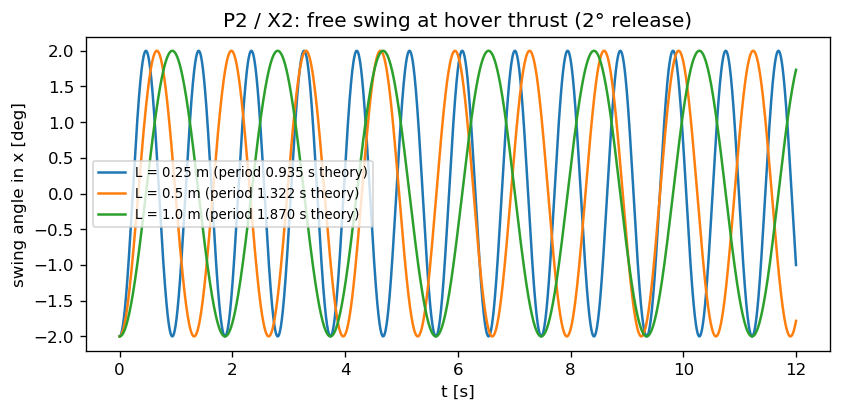
\includegraphics[width=0.78\textwidth]{figs/c1_period.png}
\caption{Gate P2: swing of the C1 payload under a hovering drone for three cable lengths, compared with the two-body
pendulum period.}
\label{fig:c1period}
\end{figure}

\textbf{Trajectories and metrics (M1--M5).} Reference trajectories are built from polynomials and complex exponentials
so that derivatives up to sixth order are analytic; they agree with a symbolic (sympy) oracle to $1.4\times10^{-11}$
relative error. Metrics are verified on signals with known answers, and the logger is bit-reproducible.

% =====================================================================================================
\section{Phase 2: implementing Paper 1}
\label{sec:phase2impl}

\subsection{Flatness map (step 2.1, gates F1--F6)}
The flatness map is exact at hover, satisfies the equations of motion with a residual of $10^{-14}$, and its
derivatives converge at the expected rate. As an independent check it agrees with Udaan, an open-source implementation of
the same map, to $1.1\times10^{-13}$. The strongest test is an \emph{open-loop replay}: the drone is placed exactly on the
flat state of a reference and the flatness wrench is applied with no feedback. The real MuJoCo dynamics then follow the
reference within 1~cm for 3 to 6~s before the unstable error growth takes over (\Cref{fig:flat}). This confirms that the
map, the X2 model and the actuator chain are mutually consistent.

\begin{figure}[htbp]
\centering
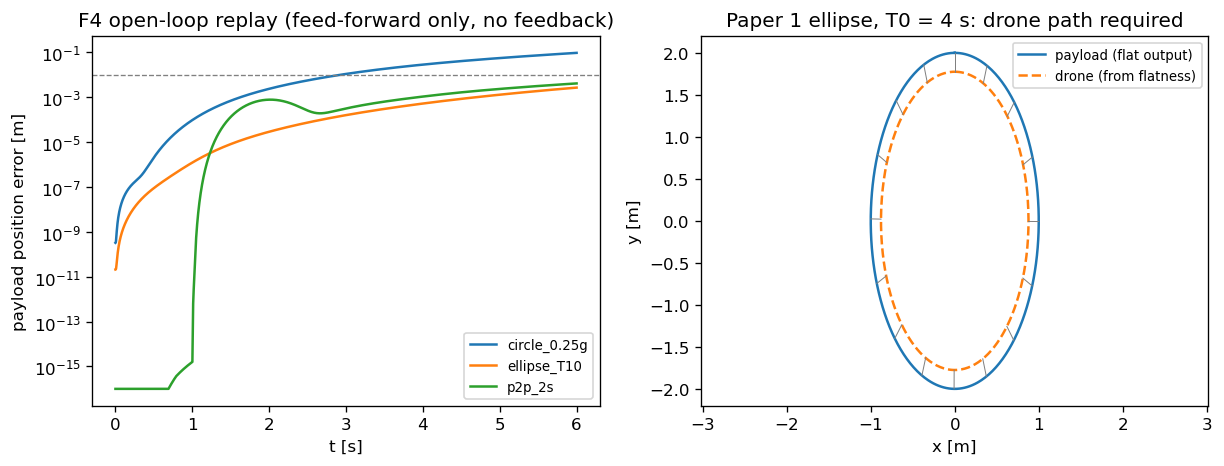
\includegraphics[width=0.85\textwidth]{figs/flatness.png}
\caption{Step 2.1: open-loop replay of flatness wrenches in MuJoCo for several references, and the derivative
convergence checks.}
\label{fig:flat}
\end{figure}

\subsection{Choosing the gains (finding F3)}
\label{sec:gains}
Paper~1 does not publish usable gains for this drone. We parametrise the three loops by their bandwidths
$\omega_x,\omega_q,\omega_R$ and damping ratio $\zeta=0.9$:
\[
k_x = (m_Q{+}m_L)\,\omega_x^2,\; k_v = 2\zeta(m_Q{+}m_L)\,\omega_x,\quad
k_q = m_Q l\,\omega_q^2,\; k_\omega = 2\zeta m_Q l\,\omega_q,\quad
K_R = \omega_R^2 J,\; K_\Omega = 2\zeta\omega_R J .
\]
Scaling the attitude gains by the inertia gives every axis the same bandwidth. Two constraints then fix the values.

\textbf{Separation.} With only $3\times$ between loops (2 / 6 / 20~rad/s) the coupled system is lightly damped: a 1~m
step settles in 3.65~s instead of the 2.13~s predicted by the linear design. With $2\times$ it oscillates indefinitely, and a
cable loop only $3\times$ below the attitude loop (10 / 30) is unstable. With at least $5\times$ the closed loop matches
the linear prediction.

\textbf{Rotor limits.} At 40--60~rad/s attitude bandwidth a $30^\circ$ swing saturates the X2 rotors on almost every
tick and the drone diverges, while the same gains converge with unlimited thrust. About 30~rad/s is therefore the
ceiling.

\begin{keybox}[title={F3: gains used throughout Phase 2}]
$\omega_x,\omega_q,\omega_R = 1.5,\;7.5,\;30$ rad/s, i.e.\ $k_x = 3.43$, $k_v = 4.12$, $k_q = 37.3$, $k_\omega = 8.94$,
$\mathrm{diag}(K_R) = (33.0, 22.9, 54.5)$, $\mathrm{diag}(K_\Omega) = (1.98, 1.37, 3.27)$ in SI units.
The time-scale separation that the theory needs and the thrust the X2 has leave very little room: these are the
fastest gains that satisfy both.
\end{keybox}

\subsection{Controller gates (step 2.2, K1--K7)}
\label{sec:k-gates}
Gates that test the theory itself (K1, K2, K5) use an \emph{ideal actuator} option that removes rotor limits, because
Paper~1 assumes unlimited inputs. The others use the real X2 limits.

\begin{table}[htbp]
\centering\small
\begin{tabularx}{\textwidth}{@{}l X X@{}}
\toprule
Gate & Test & Result \\
\midrule
K1 & Attitude mode, $60^\circ$ initial error & error decays at 28.4/s vs 27/s predicted \\
K2 & Cable-attitude mode, $120^\circ$ initial cable error & decays at 7.6/s vs 6.75/s predicted \\
K3 & Position mode, 1~m step & settles in 2.87~s vs 2.83~s from linear design \\
K4 & Tracking T1 2~s, T2 $0.5g$, T3 10~s & max error $\le 0.17$~mm \\
K5 & Faster attitude loop (15, 30, 60~rad/s) & error decreases monotonically, as singular perturbation predicts \\
K6 & Cable-rate error form & tangent to $S^2$; the wrong (angular-velocity) form leaves a $179^\circ$ residual swing \\
K7 & Source of command derivatives & flatness 0.05~mm, numerical differentiation 12.5~mm, zero 0.67~m RMSE \\
\bottomrule
\end{tabularx}
\caption{Step 2.2 controller gates.}
\end{table}

K7 is worth stressing: the feed-forward from the flatness map is not a refinement but a requirement. Without it the
same controller misses a circle by more than half a metre.

\begin{figure}[htbp]
\centering
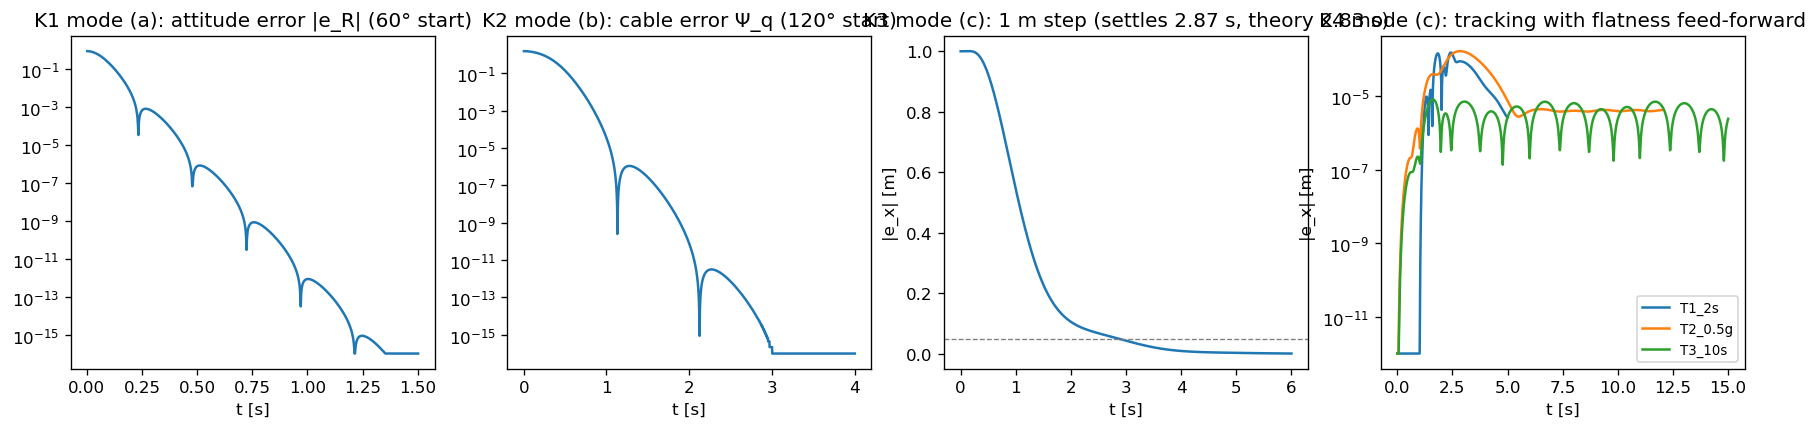
\includegraphics[width=0.95\textwidth]{figs/geometric.png}
\caption{Step 2.2: attitude-mode decay (K1), cable-mode decay (K2), 1~m step (K3) and tracking errors (K4).}
\end{figure}

% =====================================================================================================
\section{Experiments with Paper 1}
\label{sec:experiments}

\subsection{E1.1 The flatness study on the ellipse (step 2.3)}

\textbf{Setup.} Paper~1's Fig.~3 uses the load trajectory
$x_L(t) = (A_x\sin\tfrac{2\pi t}{T_0},\; A_y\cos\tfrac{2\pi t}{T_0},\; A_z)$ with $\psi=0$ and periods $T_0$ from 10~s
down to 1~s. We use $A_x\times A_y = 0.5\times1.0$~m as the main case, $1.0\times2.0$~m as a second case, and $A_z$ at the
payload's hover height. The study has three parts: (A) reproduce Fig.~3 from the flatness map; (B) find, by bisection on
$T_0$, the shortest period for which every rotor thrust required by the flatness map stays in 0--13~N; (C) run the
closed loop for three full periods on the X2 and with the ideal actuator, starting exactly on the flat state.

\textbf{Part A.} The load path is identical for every $T_0$; the drone paths are not (\Cref{fig:fig3}). As $T_0$
decreases the drone flies a smaller, lower, peanut-shaped path \emph{inside} the load's ellipse, because the load swings
outward and the drone has to lean against it. Peak tilt grows from $20^\circ$ at 3~s to $54^\circ$ at 1.5~s and exceeds
$90^\circ$ below about 1.25~s, where the drone would have to fly partly upside down. Our first gate assumed the drone's
path grows with speed; the simulation showed the opposite, and the gate was replaced by ``required tilt and torque grow
as $T_0$ decreases''.

\begin{figure}[htbp]
\centering
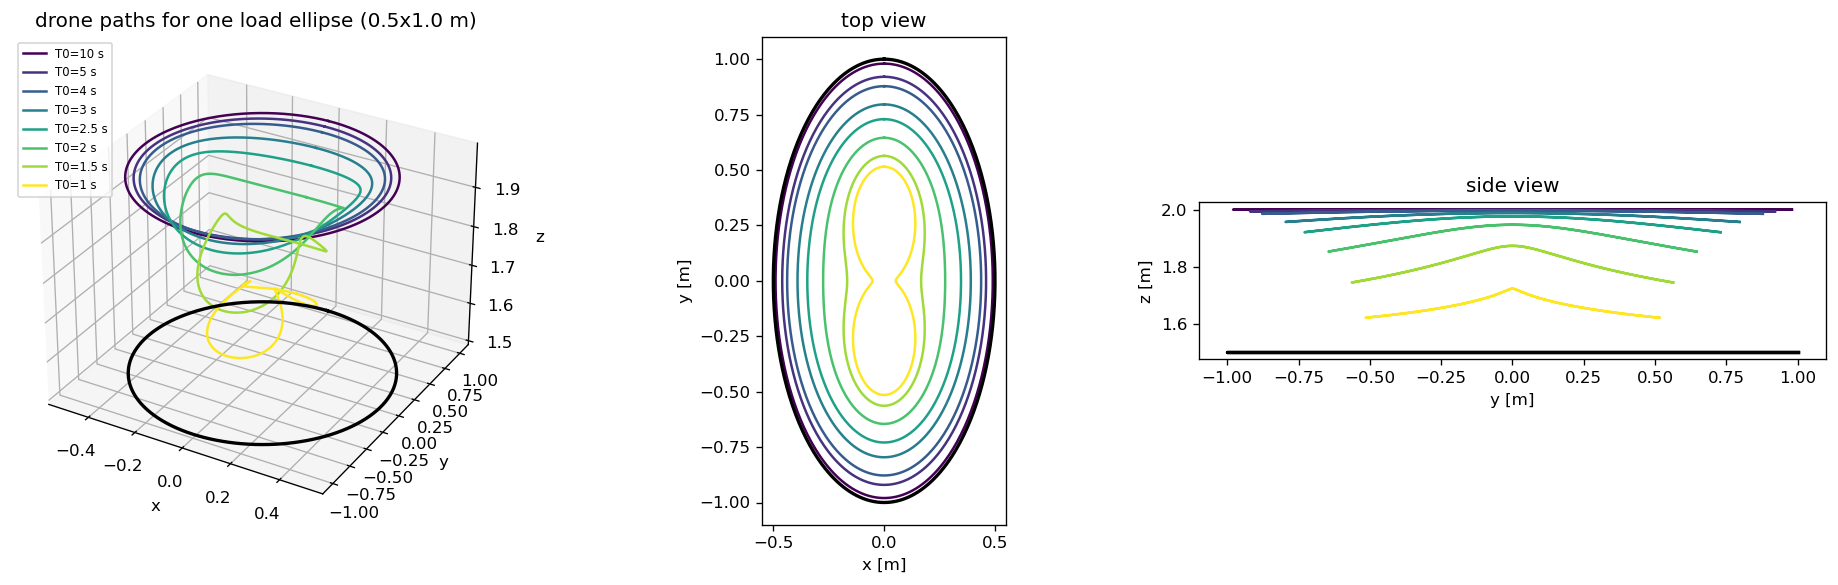
\includegraphics[width=0.95\textwidth]{figs/A_fig3_reproduction.png}
\caption{Paper~1 Fig.~3 reproduced: drone paths (colour) required for one load ellipse (black), $T_0=10\ldots1$~s.}
\label{fig:fig3}
\end{figure}

\textbf{Part B.} \Cref{tab:tcrit} gives the feasibility boundary. Below it the required thrust explodes: at $T_0=1.5$~s
the flatness map asks for thousands of newtons per rotor. Across a size sweep ($A_y$ from 0.25 to 3~m at aspect 1:2)
$T_0^\ast$ grows monotonically from 1.35~s to 2.92~s.

\begin{table}[htbp]
\centering\small
\begin{tabular}{@{}lccc@{}}
\toprule
Ellipse & $T_0^\ast$ & Load peak speed & Load peak acceleration \\
\midrule
$0.5\times1.0$ m & 2.12 s & 3.0 m/s & 8.8 m/s$^2$ \\
$1.0\times2.0$ m & 2.61 s & 4.8 m/s & 11.6 m/s$^2$ \\
\bottomrule
\end{tabular}
\caption{X2 feasibility boundary on Paper~1's ellipse (rigid cable 0.5~m, payload 0.2~kg).}
\label{tab:tcrit}
\end{table}

\textbf{Part C.} Above $T_0^\ast$ the X2 behaves exactly like the ideal actuator, with no saturation, and errors range from
1~$\mu$m at 10~s to about 1.6~mm close to the boundary. Slightly below it (2.0~s for the main ellipse, 2.5~s for the
second) the rotors saturate on 42--51\% of ticks, yet the prioritised mixer keeps the error below 1.7~mm. Further below,
the X2 diverges. At $T_0=1.5$~s \emph{even the ideal actuator fails} (19~cm and 2.2~m errors): the reference needs about
62~rad/s body rates, which a 30~rad/s attitude loop cannot follow (\Cref{fig:closedloop}).

\begin{figure}[htbp]
\centering
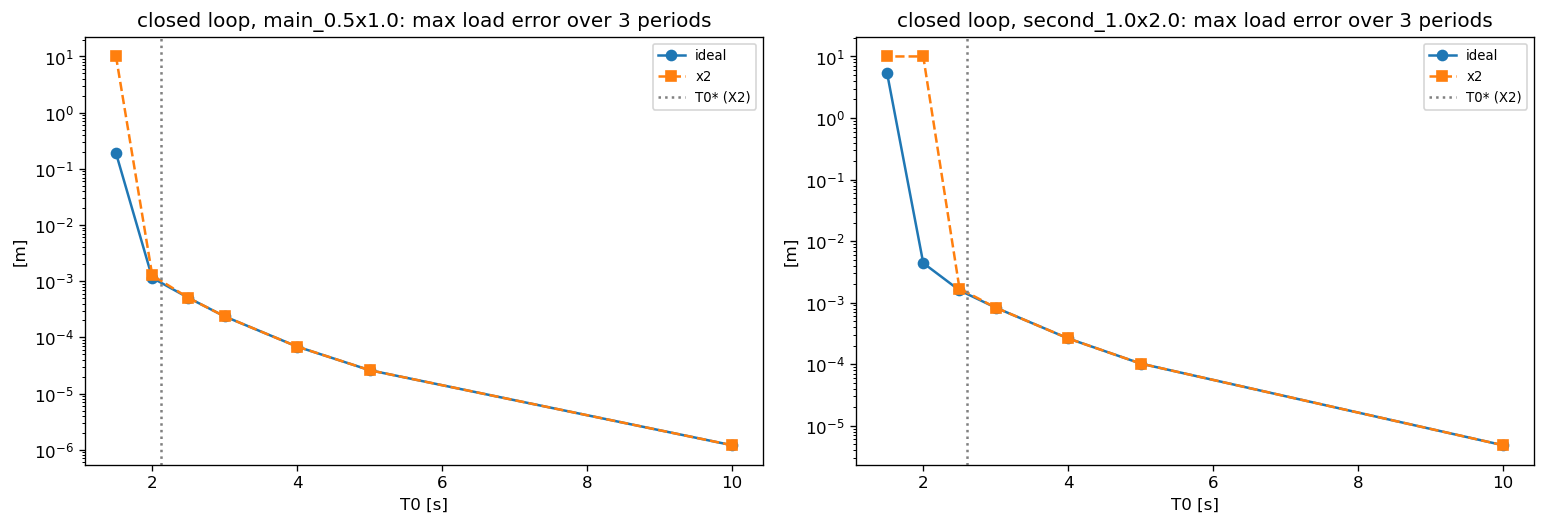
\includegraphics[width=0.85\textwidth]{figs/C_closed_loop.png}
\caption{Closed-loop maximum load error over three periods vs $T_0$, X2 and ideal actuator; dotted line: $T_0^\ast$.}
\label{fig:closedloop}
\end{figure}

\begin{keybox}[title={F4: two speed limits}]
The X2 can fly Paper~1's ellipse only down to $T_0^\ast = 2.12$~s ($0.5\times1.0$~m), a load speed of 3~m/s. A second,
lower limit comes from the controller: with attitude bandwidth capped at 30~rad/s by F3, references faster than about
1.5~s cannot be tracked even with unlimited thrust.
\end{keybox}

\subsection{E1.2 Recovery from a near-flipped start (step 2.4)}

\textbf{Setup.} Paper~1 (Figs.~4--5) starts the drone flipped $178^\circ$ about the $y$ axis, the cable at $178^\circ$ and
the load far from its reference, without giving the numbers. We rotate drone and cable by the same angle $\theta$ about
$y$, start everything at rest with the load 2~m from the reference along $(1,-1,-1)/\sqrt3$, and use the main ellipse at
$T_0=5$~s as the reference, for 10~s. Recovery means entering a 5~cm band and staying there for at least 2~s.

\textbf{Paper~1 reproduced.} With the ideal actuator and $\theta=178^\circ$ all three errors converge (\Cref{fig:rec}):
the load is inside 5~cm at 5.1~s, the final error is 0.07~mm, and the drone loses 0.72~m of height. The tension plot shows
something the paper does not discuss: for about the first second the rigid link \emph{pushes} the load (tension down to
$-2.8$~N, 9\% of the run).

\begin{figure}[htbp]
\centering
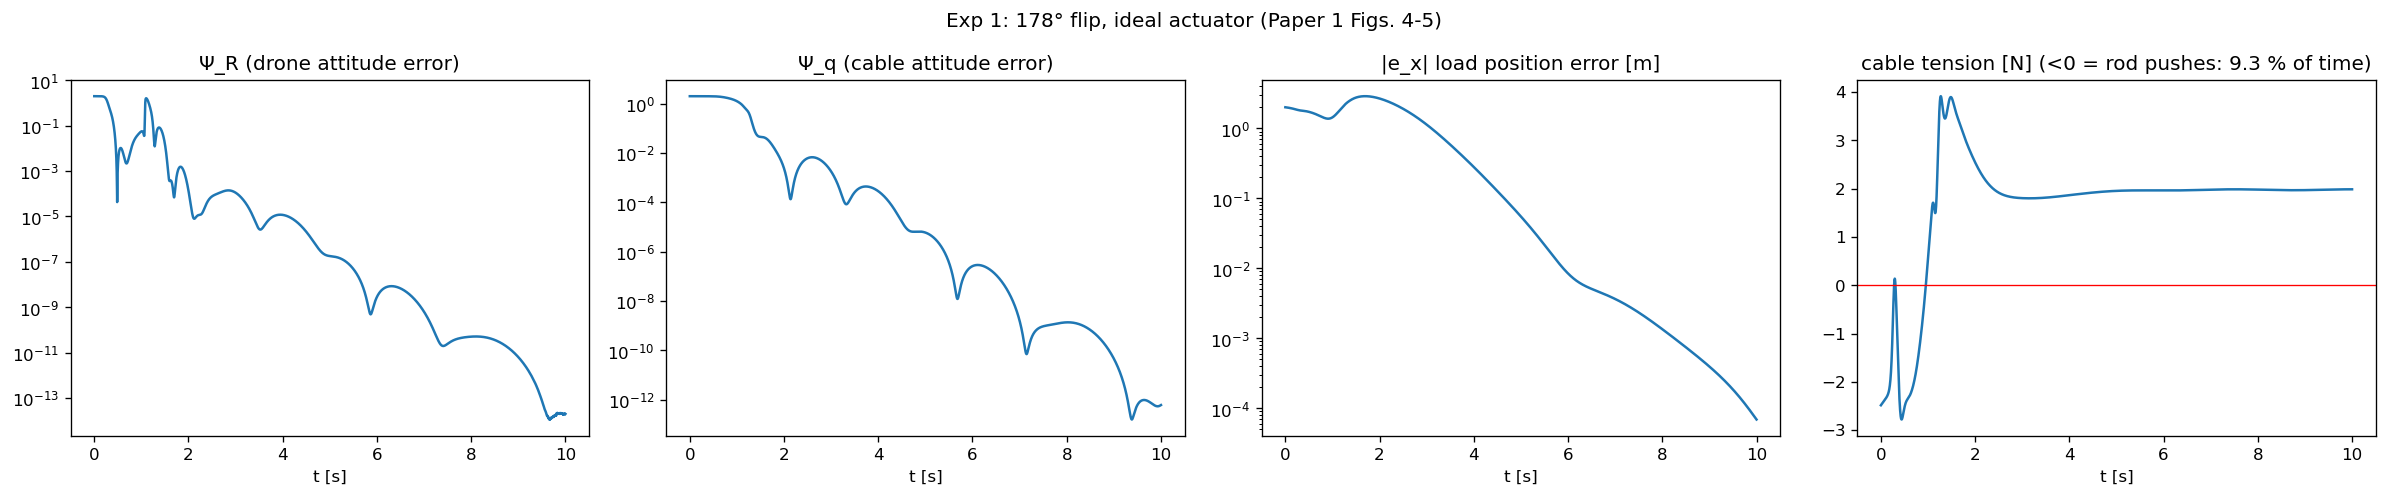
\includegraphics[width=0.95\textwidth]{figs/E1_paper1_recovery.png}
\caption{Recovery from a $178^\circ$ flip with unlimited thrust and the rigid cable: attitude, cable and position errors,
and the cable tension.}
\label{fig:rec}
\end{figure}

\textbf{On the X2.} With 0--13~N rotors the result depends on $\theta$ in an irregular way (\Cref{fig:sweep}). A 2~m
position error alone ($\theta=0$) recovers in 3.1~s with 2\% saturation, and $10^\circ$ also recovers cleanly. From
$20^\circ$ the controller demands 15--46~N\,m against roughly 2~N\,m available, the rotors are pinned at their limits, and
drone and load tumble. Outcomes then change with $1^\circ$ differences ($30^\circ$ fails, $31^\circ$ recovers); recovered
runs lose 1--9~m of height and failed runs fall up to 50~m.

\begin{figure}[htbp]
\centering
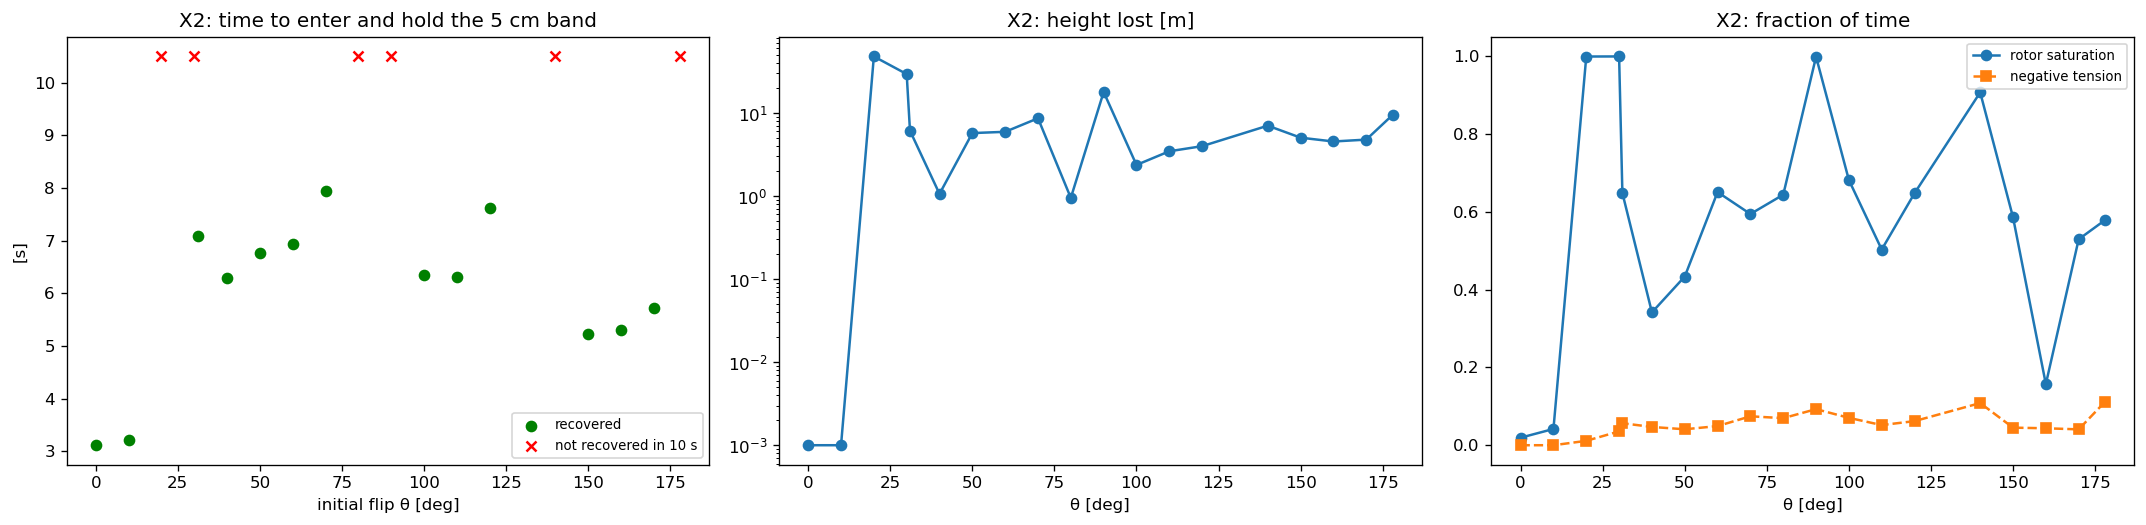
\includegraphics[width=0.9\textwidth]{figs/E2_x2_sweep.png}
\caption{X2 flip-angle sweep: recovery time (red crosses: not recovered in 10~s), height lost, rotor saturation and
negative-tension fraction.}
\label{fig:sweep}
\end{figure}

\begin{keybox}[title={F5: recovery under rotor limits}]
Paper~1's almost-global recovery relies on unlimited torque and on a cable that can push. On the X2, recovery from flips
of $20^\circ$ or more is unreliable (chaotic in the initial angle) and costs metres of height.
\end{keybox}

\subsection{E1.3 Benchmark subset T0--T3 (step 2.5)}

All 13 benchmark cases of \Cref{tab:traj} were run on the X2 and with the ideal actuator, after a feasibility pre-check
with the flatness map. Every case whose reference is feasible succeeds, and on these cases the X2 and the ideal actuator
give identical numbers: tracking errors are at most 0.45~mm on T1--T3, the $15^\circ$ and $30^\circ$ initial swings settle
in 1.6 and 2.0~s (about 1.1 and 1.4 pendulum periods), and the mass-scaled gust settles in 1.25~s. Only two cases fail:
the 1~m move in 1~s, whose reference needs $\pm570$~N per rotor, and the severe 2~N gust (a $1g$ push on a 0.2~kg payload),
which no controller can keep within the 0.5~m success limit.

The dynamic-swing metric behaves as designed: on the tracking cases the swing reaches $45^\circ$ while the dynamic swing
stays below $0.01^\circ$. All of that swing is what the trajectory requires, none is unwanted oscillation.

The original D9 gust (2~N) was revised during this step: it was replaced by $0.25g\times m_L$ so that it scales with payload
mass, and 2~N was kept as a ``severe'' level. Controller time is 1.4~ms per step in Python, including the flatness
feed-forward, which fits in the 2~ms period at 500~Hz with little margin.

\begin{figure}[htbp]
\centering
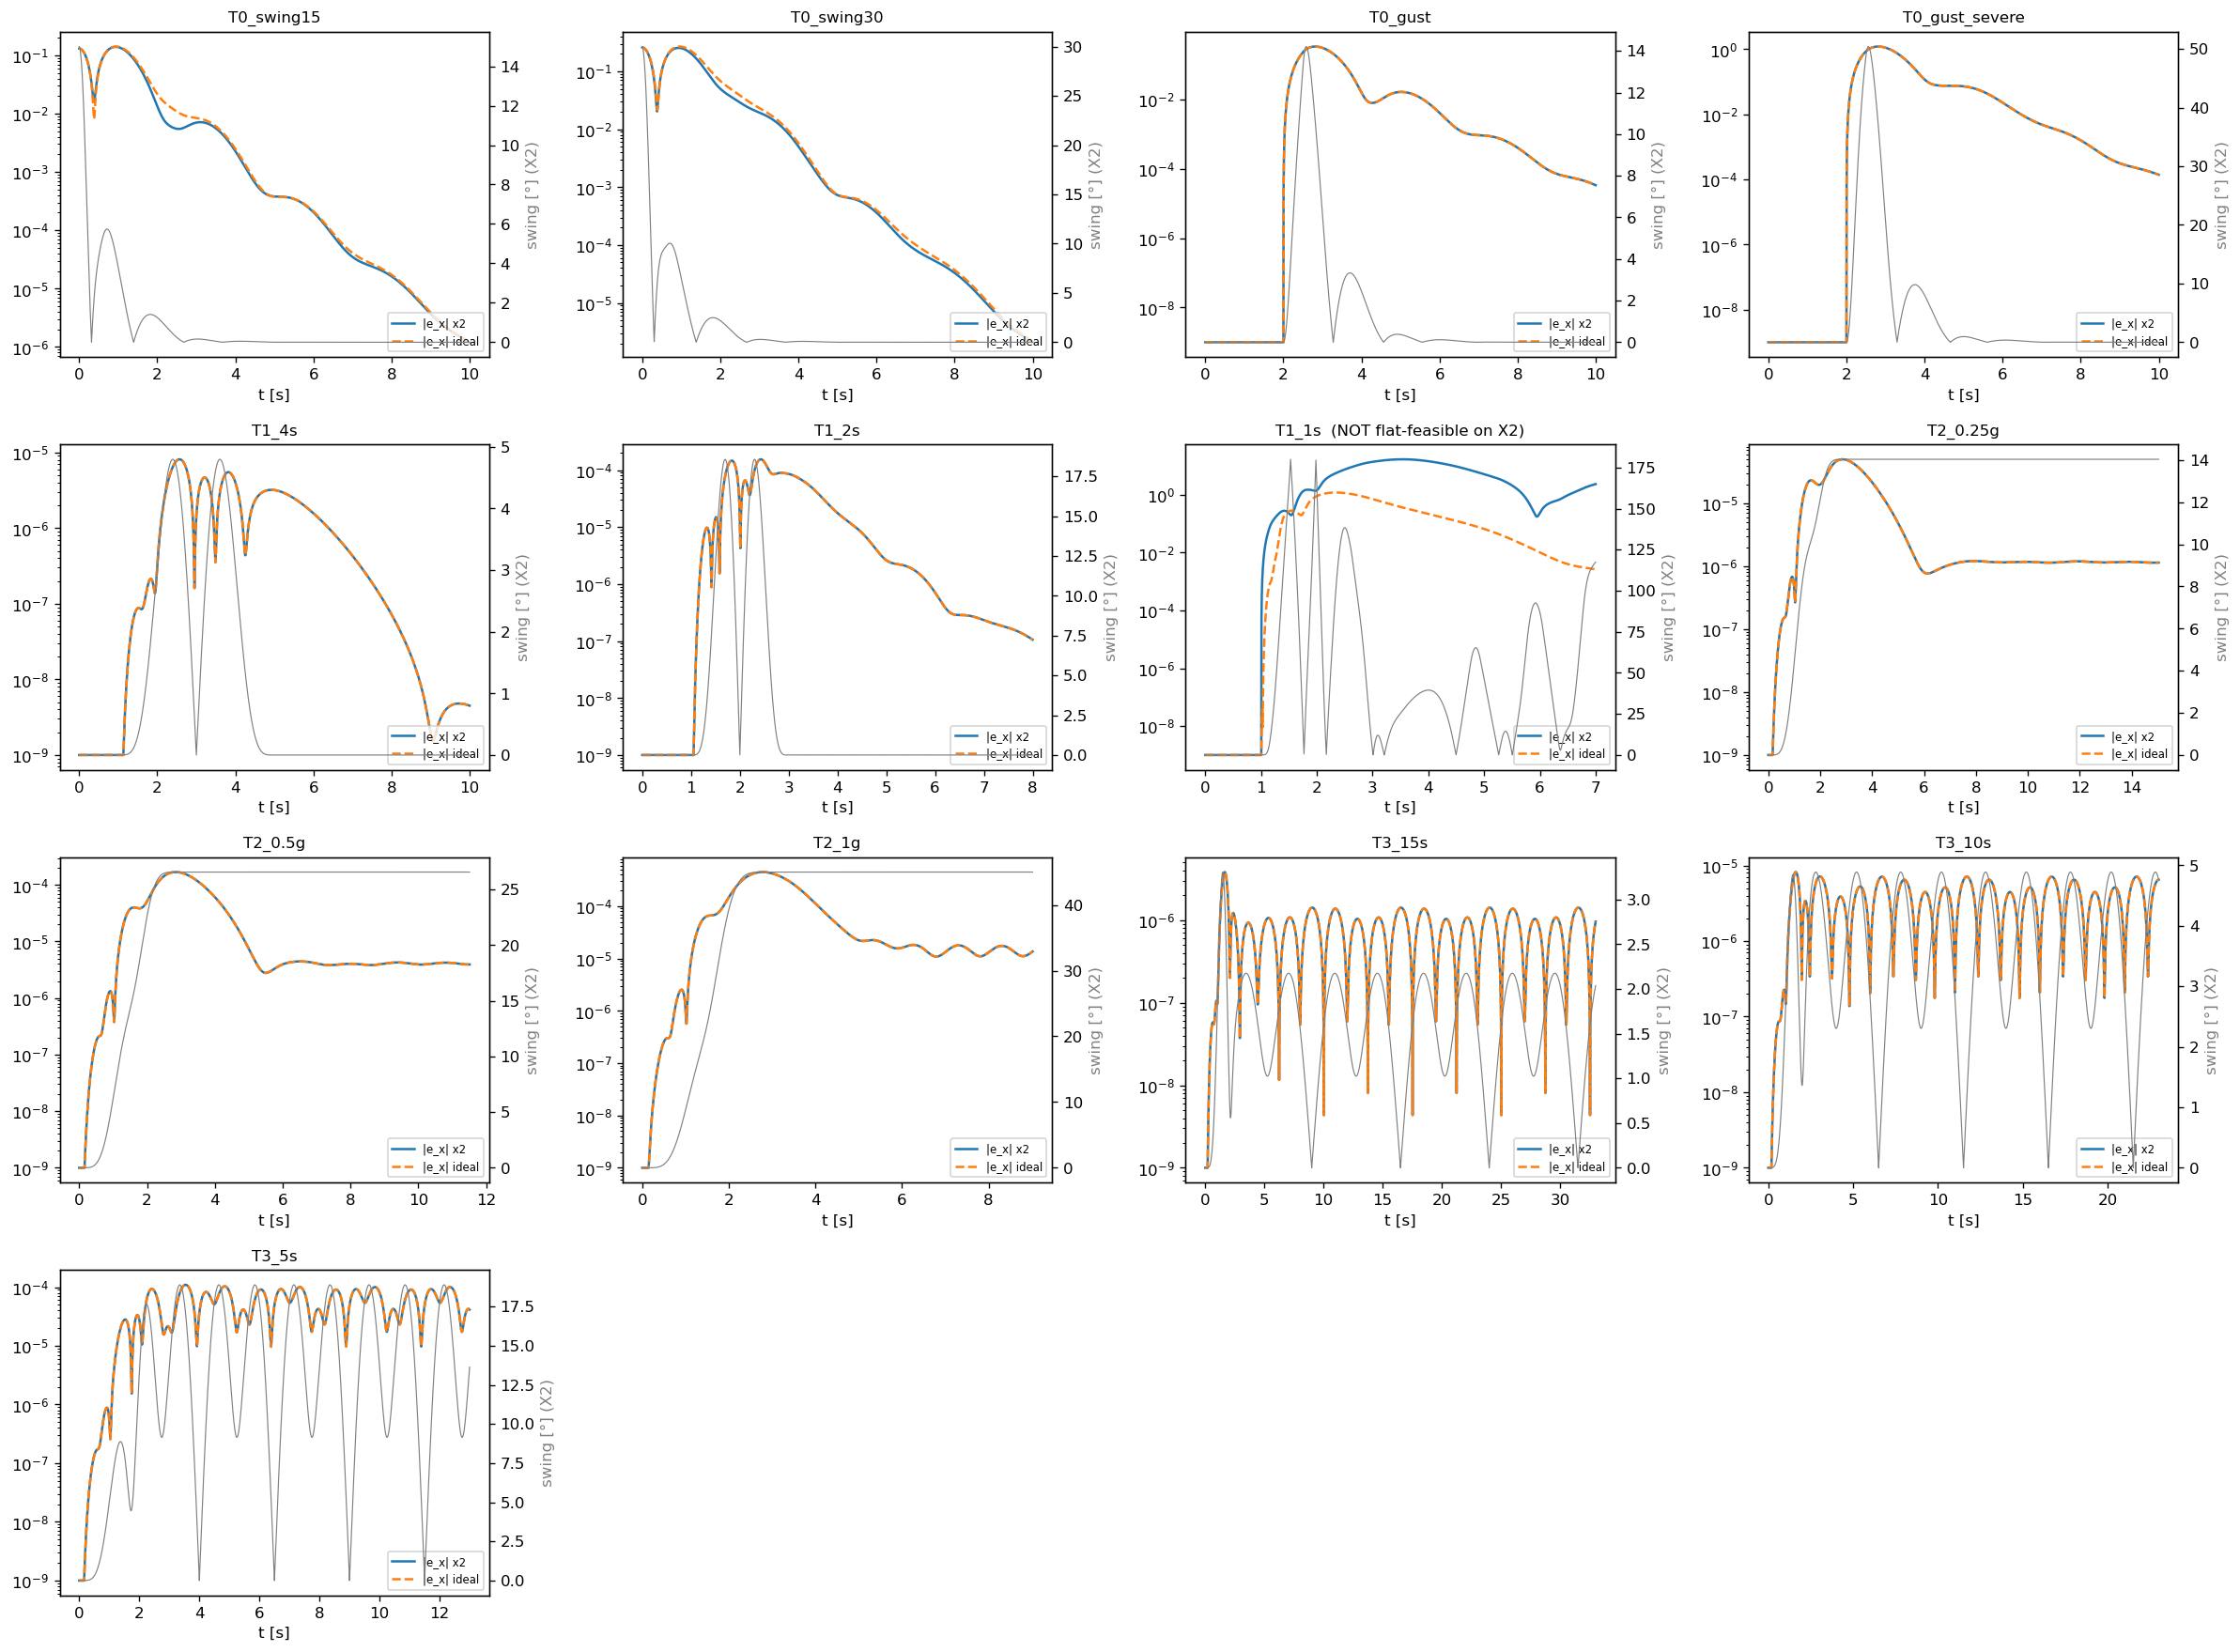
\includegraphics[width=0.95\textwidth]{figs/benchmark_T0_T3.png}
\caption{Benchmark subset: load error (log scale, solid X2, dashed ideal actuator) and swing angle (grey) for each case.}
\end{figure}

\subsection{E1.4a A cable that can go slack (step 2.6a)}
\label{sec:c2}

\textbf{Validation of C2 (gates S1--S6).} While taut, C2 reproduces C1: hover stretch 0.01~mm, swing period within
0.008\% of theory, and payload paths within 0.10~mm of C1 over a $30^\circ$ swing. When the payload is thrown upward at
3~m/s it goes slack twice, the tension is exactly zero while slack, the payload follows a ballistic arc (acceleration
error $2\times10^{-10}$), and the tension is never negative.

\begin{cavbox}[title={F6: what a snap means in an inextensible cable}]
When a slack inextensible cable becomes taut it stops the payload's relative motion instantly: physically this is an
impulse, with no finite peak force. The peak tension MuJoCo reports (186 to 509~N) is set only by the softness of the
constraint and the timestep, so it is not a physical result and is never reported for C2. The \emph{impulse} is physical
(about 0.64~N\,s, the payload's momentum change); it converges between 0.5 and 0.25~ms (3\%) but is under-resolved by about
20\% at 1~ms. C2 runs therefore use a 0.5~ms timestep (an agreed exception to D5). Realistic snap forces need an elastic
cable (C3, Paper~3).
\end{cavbox}

\begin{figure}[htbp]
\centering
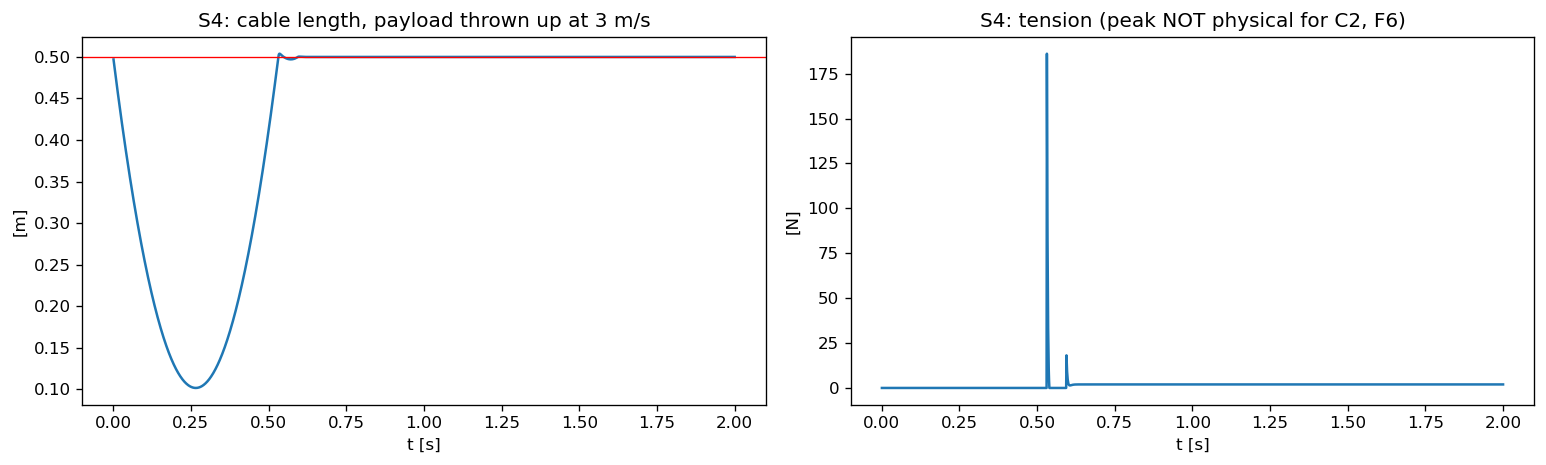
\includegraphics[width=0.8\textwidth]{figs/c2_slack_retaut.png}
\caption{Gate S4: cable length and tension when the payload is thrown upward at 3~m/s from hover.}
\end{figure}

\label{sec:c2-exp}
\textbf{Paper~1 on C2.} On every benchmark case where the cable stays taut, C2 gives the same result as C1 within 0.03~mm.
In the T5(a) test (payload thrown up at 3~m/s) the cable is slack for 0.88~s, the payload passes above the drone, and the
controller still recovers (maximum error 0.46~m, settled in 2.44~s). The decisive result is the $178^\circ$ recovery:
\emph{with unlimited thrust it now diverges}. With the load above the drone and the cable slack, thrust no longer acts on
the load; the controller keeps commanding it, the unlimited actuator launches the drone about 21~m in 0.1~s, the cable
snaps taut at over 100~N and the run diverges. On the X2 the flip sweep recovers in 7 of 19 angles instead of 14 of 19.
The descent faster than $g$ of T5(b) cannot even be posed: its reference makes the required tension negative, which is
exactly where the flatness map is singular.

\begin{figure}[htbp]
\centering
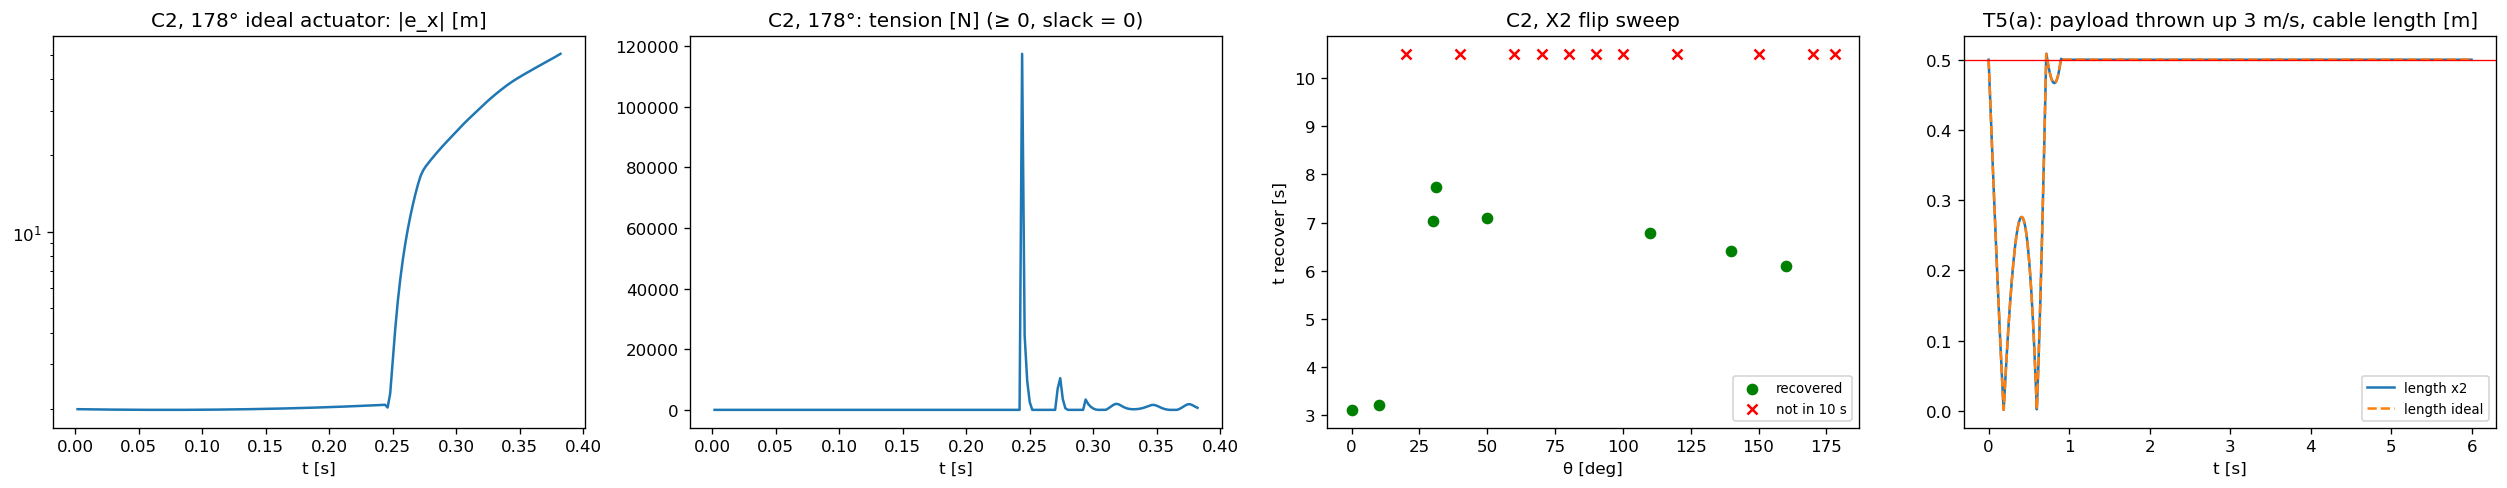
\includegraphics[width=0.95\textwidth]{figs/paper1_on_c2.png}
\caption{Paper~1 on the slack-capable cable: divergence of the $178^\circ$ recovery with unlimited thrust, the X2 flip
sweep, and the T5(a) throw test.}
\end{figure}

\begin{keybox}[title={F7: the always-taut assumption}]
Paper~1's controller is fine while the cable is taut and survives a short slack phase, but its large-angle recovery
relies on the cable being able to push the load.
\end{keybox}

\subsection{E1.4b Cable length (step 2.6b)}

The benchmark and the feasibility boundary were repeated with cable lengths of 0.25~m and 1.0~m, keeping the same
bandwidths. The concern before the run was the short cable: its free swing frequency (6.7~rad/s) is close to the
7.5~rad/s cable loop, which could break time-scale separation. It did not: 0.25~m succeeds on every feasible case. The
problem appeared at 1.0~m, where the $15^\circ$ initial swing flips the X2 (30\% saturation) and the $30^\circ$ swing fails
even with unlimited thrust.

The reason is in the gain scaling. Keeping a fixed bandwidth means $k_q = m_Q l\,\omega_q^2$ grows with $l$, so the
restoring \emph{force} for the same swing angle doubles from 0.5 to 1.0~m: a $15^\circ$ swing on 1~m asks for about 19~N
sideways, which in turn asks for a large tilt and saturates the rotors.

\begin{table}[htbp]
\centering\small
\begin{tabular}{@{}lccc@{}}
\toprule
& 0.25 m & 0.5 m & 1.0 m \\
\midrule
Free swing frequency & 6.7 rad/s & 4.7 rad/s & 3.4 rad/s \\
$T_0^\ast$, main ellipse & 1.94 s & 2.12 s & 2.26 s \\
T0 $15^\circ$ swing (X2) & settles 1.8 s & settles 1.6 s & crash \\
T0 $30^\circ$ swing (X2) & settles 2.2 s & settles 2.0 s & crash (ideal actuator also fails) \\
Feasible tracking cases & all succeed & all succeed & all succeed \\
\bottomrule
\end{tabular}
\caption{Effect of cable length with unchanged bandwidths (finding F8).}
\end{table}

Two smaller observations: a longer cable lowers the X2's maximum speed ($T_0^\ast$ increases), and the flatness
feasibility check is conservative, since at 1.0~m two cases flagged as infeasible (T1 2~s and T2 $1g$) were still tracked
with brief saturation.

\subsection{E1.4c Realistic actuation and sensing (step 2.6c)}

\textbf{A linear pre-check.} For one attitude axis with a 35~ms motor lag, the PD loop $J\ddot\theta = \tau$ has the
characteristic polynomial $\tau_m s^3 + s^2 + 2\zeta\omega_R s + \omega_R^2$. \Cref{tab:lag} shows its least-damped
pole, with and without an extra 10~ms delay (first-order Pad\'e). At our 30~rad/s the loop is barely damped with lag and
unstable with lag plus delay. A lag-compatible attitude loop has to be near 10~rad/s, which with $5\times$ separation puts
the cable loop near 2~rad/s, below the 4.7~rad/s swing it is supposed to control.

\begin{table}[htbp]
\centering\small
\begin{tabular}{@{}ccc@{}}
\toprule
$\omega_R$ & lag 35 ms: min damping & lag + 10 ms delay \\
\midrule
10 rad/s & 0.55 & 0.40 \\
15 rad/s & 0.36 & 0.20 \\
20 rad/s & 0.26 & 0.08 \\
30 rad/s & 0.13 & unstable \\
\bottomrule
\end{tabular}
\caption{Least-damped pole of the attitude loop with motor lag.}
\label{tab:lag}
\end{table}

\textbf{New components and their gates (R1--R8).} This step added the sensor and delay models, a body-rate controller and
a single closed-loop runner. Noise statistics match the specification within 1\%; the delay is exact; the new runner
reproduces step~2.5 bit for bit when all effects are off; the rate loop's step response has a 17.5~ms time constant
against 18.5~ms designed. The body-rate interface is mathematically equal to Paper~1's attitude law
(to $10^{-14}$~N\,m) except for the feed-forward torque $J R^\top R_c\dot\Omega_c$, which a thrust-plus-rates command
cannot carry: dropping it raises the T2 tracking error from 0.17~mm to about 3~mm (F9). The payload drag was set to a
smooth sphere's $C_D = 0.47$, since MuJoCo's default formula gives an effective $C_D$ of 1.0.

\textbf{One factor at a time.} Each effect was switched on alone, then all together, on the 11 feasible benchmark cases,
with two gain sets: Paper~1's nominal 1.5 / 7.5 / 30 and a lag-compatible 0.4 / 2 / 10~rad/s. Noisy settings use 20 seeds,
for 990 runs in total.

\begin{figure}[htbp]
\centering
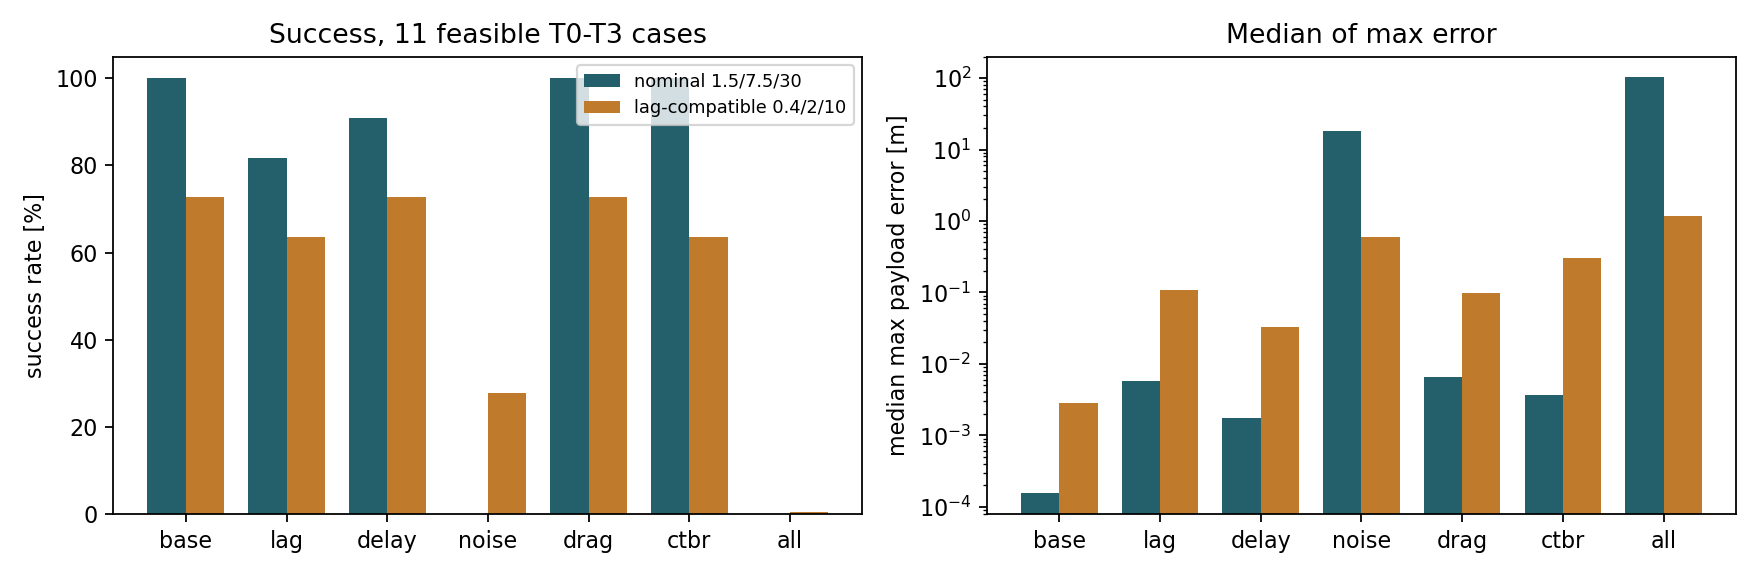
\includegraphics[width=0.95\textwidth]{figs/realism_ofat.png}
\caption{Success rate and median maximum error per setting: base (L0), motor lag 35~ms, delay 10~ms, sensor noise, drag,
CTBR interface at 100~Hz, and all together.}
\label{fig:ofat}
\end{figure}

With the nominal gains, delay, drag and the body-rate interface cost little (91--100\% success). Motor lag gives 82\%:
it breaks only the swing-recovery cases (errors of 45 and 170~m), while all eight tracking cases still succeed.
Sensor noise is decisive: \emph{all 220 noisy runs crash}, and so do all 220 runs with every effect on. A per-channel test
at hover isolates the cause:

\begin{table}[htbp]
\centering\small
\begin{tabular}{@{}lccl@{}}
\toprule
Noise channel (D10 level) & Max error & Saturation & Outcome \\
\midrule
Position 1 cm & 0.41 m & 40\% & survives, poorly \\
Velocity 5 cm/s & 2.4 m & 96\% & crash (tilt $173^\circ$) \\
Attitude $1^\circ$ & 2.4 mm & 82\% & survives \\
Gyro 0.05 rad/s & 0.25 mm & 9\% & fine \\
All channels $\times 0.1$ & $\le$ 0.7 mm & $\approx 0$ & fine \\
\bottomrule
\end{tabular}
\caption{Hover with one noise channel at a time, nominal gains.}
\end{table}

Paper~1 forms the cable rate as $\dot q = (v_L - v_Q)/l$ from two raw velocities, which gives about 0.14~rad/s of noise.
The cable loop multiplies it and the 30~rad/s attitude loop turns it into large torque commands; the rotors saturate and
the drone flips. The lag-compatible gains never crash, but they cannot damp a $30^\circ$ swing even at L0 (3.5~m error),
reach only 73\% success at L0 and 0\% with every effect on.

\begin{keybox}[title={F10: realistic sensing and actuation}]
Under realistic sensing Paper~1 is unusable without a state estimator, and velocity noise is the main cause. Motor lag
breaks swing recovery. The two cannot be fixed together by retuning: gains slow enough for the lag are too slow to damp
the swing.
\end{keybox}

\begin{cavbox}[title={Caveat on the noise model}]
D10 applies white noise independently at every 500~Hz tick. Filtered motion-capture data is smoother at high frequency,
so the \emph{severity} of F10 depends on this assumption. The need for some filtering does not.
\end{cavbox}

% =====================================================================================================
\section{Summary of findings}

\begin{longtable}{@{}p{0.07\textwidth}p{0.88\textwidth}@{}}
\toprule
ID & Finding \\
\midrule
\endhead
F1 & MuJoCo air drag on the X2 is quadratic and small at low speed (0.10~N at 2~m/s); real rotor drag is roughly linear and
larger. Not used as a precise model; covered by randomisation. \\
F2 & Motor lag must use MuJoCo's \code{filter} dynamics under RK4 (\code{filterexact} has 1.6~cN error); read motor state
from \code{data.act}. \\
F3 & Paper~1 needs about $5\times$ loop separation; X2 rotors cap the attitude loop near 30~rad/s; gains 1.5 / 7.5 /
30~rad/s. \\
F4 & X2 speed limit on Paper~1's ellipse: $T_0^\ast = 2.12$~s ($0.5\times1.0$~m) and 2.61~s ($1.0\times2.0$~m); at
1.5~s even unlimited thrust fails (bandwidth limit). \\
F5 & Under rotor limits, recovery from flips $\ge 20^\circ$ is chaotic and costs metres of height. \\
F6 & For an inextensible slack cable, peak snap force is numerical; the snap impulse is physical and needs a 0.5~ms step. \\
F7 & With a slack-capable cable Paper~1 tracks as before, survives a throw, but its $178^\circ$ recovery diverges: it relied
on the cable pushing. \\
F8 & Fixed-bandwidth gains scale the cable force with length: 1.0~m crashes on a $15^\circ$ swing; 0.25~m works. \\
F9 & A body-rate (CTBR) interface drops Paper~1's feed-forward torque: 0.17~mm becomes about 3~mm. \\
F10 & Velocity noise crashes Paper~1 (0/220); motor lag breaks swing recovery; lag-compatible gains cannot damp the swing. \\
\bottomrule
\caption{Findings of Phases 1 and 2. Full wording and numbers are in \code{SIMULATION\_DESIGN.md}.}
\end{longtable}

% =====================================================================================================
\section{Discussion}

\subsection{What the results say about Paper 1}
Paper~1's theory is correct and our implementation reproduces it to round-off where its assumptions hold. Its
limitations are not errors but consequences of four assumptions that a real system violates: unlimited thrust, a cable
that can push, perfect state knowledge and instantaneous actuators. The interesting result is how these assumptions
interact through the time-scale separation the stability proof needs. Separation pushes the attitude loop up; rotor limits
cap it at 30~rad/s; motor lag pushes it below about 10~rad/s; and the payload's own swing frequency sets a lower bound on
the cable loop. On the X2 there is no set of cascade gains that satisfies all four.

\subsection{Limits of this study}
The study tests Paper~1 as published: gains were not retuned per condition, on purpose, and a systematic tuning protocol
(D12) follows in Phase~3. The noise model is white per tick, as discussed above. The 35~ms motor time constant is a literature
value from another platform; the X2's is not identified, and it will be randomised. Rotor downwash on the payload and
ground effect are not modelled, as in the reference papers. All results are in simulation.

\subsection{Gaps and next steps}
The findings point to five capabilities that Paper~1 lacks: control that respects rotor limits (F3--F5), recovery that
knows the cable can only pull (F7), state estimation (F10), gains or structures that hold across cable lengths (F8), and
swing damping that is compatible with motor lag (F10). Phase~3 turns the survey (Paper~2) into baseline controllers and the
tuning protocol; Phase~4 tests Paper~3, whose LQR with output weighting and Kalman filter on an elastic cable addresses
part of these gaps directly. A contribution can be built on the combination that none of the reviewed controllers covers:
actuator- and slack-aware control with estimation, evaluated on this benchmark.

% =====================================================================================================
\appendix
\section{Reproducing the results}
\label{app:reproduce}
All commands run from the repository root with the system Python 3 (MuJoCo 3.17, NumPy, Matplotlib, PyYAML). Each
experiment creates \code{results/<phase>/<experiment>/<timestamp>/} with \code{config.yaml}, \code{meta.json}
(including the git commit), \code{metrics.json}, \code{data.npz}, figures and a README.

\begin{table}[H]
\centering\small
\begin{tabularx}{\textwidth}{@{}l X@{}}
\toprule
Command & Produces \\
\midrule
\code{scripts/test.sh} & all 66 tests (about 6 minutes) \\
\code{python3 experiments/e11\_x2\_validation.py} & drone gates G1--G5 \\
\code{python3 experiments/e12\_actuator\_validation.py} & actuator gates A1--A6 \\
\code{python3 experiments/e13\_c1\_p1\_validation.py} & cable C1 gates P1--P7 \\
\code{python3 experiments/e14\_trajectories\_metrics.py} & trajectory and metric gates M1--M5 \\
\code{python3 experiments/e21\_flatness.py} & flatness gates F1--F6 \\
\code{python3 experiments/e22\_geometric\_control.py} & controller gates K1--K7 \\
\code{python3 experiments/e23\_ellipse\_study.py} & E1.1, Figs.~\ref{fig:fig3}, \ref{fig:closedloop} \\
\code{python3 experiments/e24\_recovery.py} & E1.2, Figs.~\ref{fig:rec}, \ref{fig:sweep} \\
\code{python3 experiments/e25\_benchmark\_subset.py} & E1.3 results table \\
\code{python3 experiments/e26a\_c2\_validation.py} & C2 gates S1--S6 \\
\code{python3 experiments/e26a\_paper1\_on\_c2.py} & E1.4a \\
\code{python3 experiments/e26b\_cable\_length.py} & E1.4b \\
\code{python3 experiments/e26c1\_l1\_validation.py} & L1 gates R1--R8 \\
\code{python3 experiments/e26c2\_realism\_ofat.py --seeds=20 --workers=3} & E1.4c, 990 runs (about 2 hours on 3 cores; resumes from a checkpoint if stopped) \\
\bottomrule
\end{tabularx}
\end{table}

\section{Repository map}
\begin{table}[H]
\centering\small
\begin{tabularx}{\textwidth}{@{}l X@{}}
\toprule
Path & Content \\
\midrule
\code{SIMULATION\_DESIGN.md} & design decisions D1--D12, review log, findings F1--F10, sources \\
\code{IMPLEMENTATION\_PLAN.md} & working rules, step plan, progress log \\
\code{configs/base.yaml} & every parameter, each traced to a decision \\
\code{assets/skydio\_x2/} & vendored Menagerie X2 files with licence \\
\code{sim/model.py} & builds the MuJoCo model (X2, cable C1/C2, payload, drag, motor lag) \\
\code{sim/actuators.py}, \code{sim/simulator.py} & mixer with PX4 priorities; multi-rate stepping \\
\code{sim/state.py} & state in Paper~1 notation, signed cable tension \\
\code{sim/trajectories.py}, \code{sim/jet.py}, \code{sim/flatness.py} & references with exact derivatives; flatness map \\
\code{sim/controllers/geometric\_paper1.py} & Paper~1 controller \\
\code{sim/controllers/rate.py}, \code{sim/realism.py}, \code{sim/closed\_loop.py} & CTBR rate loop; noise and delay; full-stack runner \\
\code{sim/checks\_*.py}, \code{tests/} & validation gates and tests \\
\code{sim/controllers/blf\_antiswing.py} & Ding, Sun \& He (2023) barrier-Lyapunov controller, contributed by L.~Alsheikh (Phase~3 work, not part of this report) \\
\bottomrule
\end{tabularx}
\end{table}

\section{Glossary}
\begin{description}[leftmargin=0pt, itemsep=2pt]
\item[Underactuated] fewer independent inputs than degrees of freedom; here the cable angles have no input.
\item[Differential flatness] all states and inputs are functions of a few outputs and their derivatives.
\item[Geometric control] control designed directly on the manifolds $SO(3)$ and $S^2$, avoiding Euler-angle singularities.
\item[Time-scale separation] nested loops with well separated bandwidths, so that inner loops can be treated as instantaneous.
\item[CTBM / CTBR] collective thrust with body moments / with body rates; two standard command interfaces.
\item[Mixer] maps thrust and moments to individual rotor thrusts and handles saturation.
\item[Feasibility boundary $T_0^\ast$] shortest ellipse period whose flatness-required rotor thrusts all lie in 0--13~N.
\item[Dynamic swing] angle between the actual cable direction and the one the flatness map predicts for the reference.
\end{description}

% =====================================================================================================
\begin{thebibliography}{9}\small
\bibitem{sreenath2013} K.~Sreenath, T.~Lee, V.~Kumar, ``Geometric control and differential flatness of a quadrotor UAV
with a cable-suspended load,'' \emph{IEEE Conference on Decision and Control}, 2013.
\bibitem{lee2010} T.~Lee, M.~Leok, N.~H.~McClamroch, ``Geometric tracking control of a quadrotor UAV on SE(3),''
\emph{IEEE Conference on Decision and Control}, 2010.
\bibitem{todorov2012} E.~Todorov, T.~Erez, Y.~Tassa, ``MuJoCo: A physics engine for model-based control,''
\emph{IEEE/RSJ IROS}, 2012.
\bibitem{menagerie} MuJoCo Menagerie: a collection of high-quality simulation models for MuJoCo, Google DeepMind,
\url{https://github.com/google-deepmind/mujoco_menagerie}.
\bibitem{faessler2018} M.~Faessler, A.~Franchi, D.~Scaramuzza, ``Differential flatness of quadrotor dynamics subject to
rotor drag for accurate tracking of high-speed trajectories,'' \emph{IEEE Robotics and Automation Letters}, 2018.
\bibitem{kaufmann2022} E.~Kaufmann, L.~Bauersfeld, D.~Scaramuzza, ``A benchmark comparison of learned control policies
for agile quadrotor flight,'' \emph{IEEE ICRA}, 2022.
\bibitem{tolba2025} Tolba, Shirinzadeh, \emph{Robotics and Autonomous Systems} 193 (2025) 105060 (Paper~3).
\bibitem{ding2023} F.~Ding, C.~Sun, S.~He, ``Anti-swing control for quadrotor-slung load transportation system with
underactuated state constraints,'' \emph{Sensors} 23 (2023) 8995.
\end{thebibliography}

\end{document}
